In our era technology has a foundamental role in almost every field. From the simple communications activities to those related to medical researches, technology is something we cannot do without. It is also a great opportunity in educational field, where it is demonstrated that the so called "stealth learning" (i.e. the help of technologies in educational scope) \cite{Sharp} is a solution to create a greater emotional involvement and that has as a consequence the ability to increase learner's learning opportunities. In our specific case, stealth learning is suitable for the treatment of patients affected by NDD to develop their cognitive, emotional and intellectual skills.
\section{Modern technologies for NDD people}
All the new existing technologies are now helping therapists and families to deal with neurological disabilities. In fact, in addition to virtual reality, smart objects, multisensor environments or smart spaces and conversational agents are used.\\
Smart objects are devices that can interact not only with the user but also with other similar devices and with the surrounding environment. Physical world can be described in terms of three properties \cite{Smart}: awareness (is a smart object to be able to understand events and human activities occurring in the physical world), representation (refers to a smart object's application and programming model) and interaction (denotes the object's ability to converse with the user in terms of input, output, control, and feedback).\\
Examples are Dolphin Sam \cite{Dolphin} and  Huggable \cite{Huggable}. \\
Smart spaces or multisensor environments are rooms in which children can play or interact in a controlled way because they are equipped with techonological items like cameras, smart objects, leds and projectors.
\\
Examples are Magic K room e M4All \cite{M4all}. \\
Conversational agents are devices that can communicate with the user in a manner consistent with what is required: an interaction of the user is answered by the agent who must be with sense.\\
\begin{figure}[H]
\centering
\begin{minipage}[c]{.40\textwidth}

\includegraphics[width=1\textwidth]{immagini/delfino.png}
\end{minipage}%
\hspace{10mm}%
\begin{minipage}[c]{.40\textwidth}
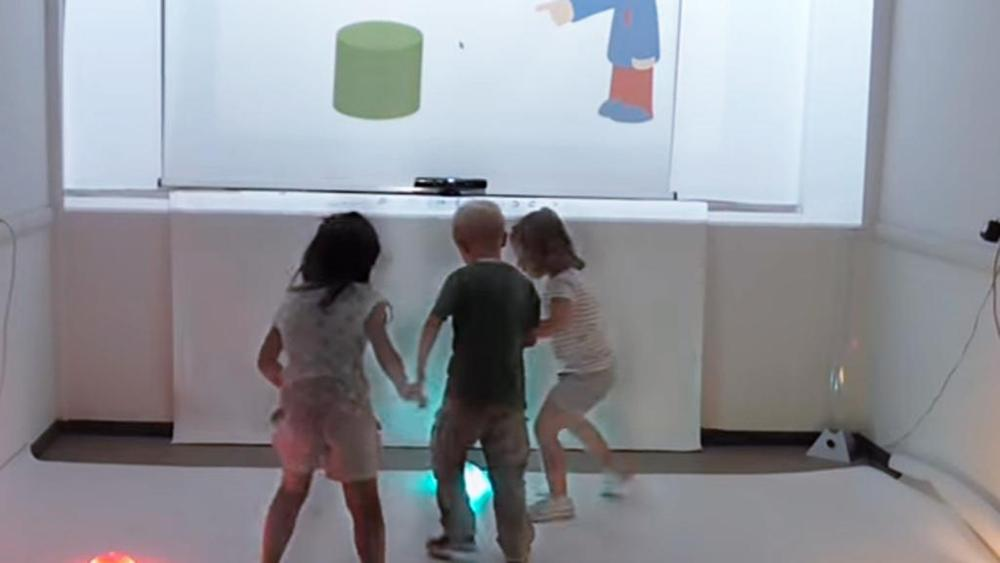
\includegraphics[width=1\textwidth]{immagini/stanzamagica.jpg}
\end{minipage}
\caption{Dolphin Sam and Magic K Room}\label{fig:smartimages}
\end{figure}
\section{Virtual Reality}
\section{Touchscreen}
The massive evolution that touchscreen devices have had in recent years, has strongly influenced our way of life. The amount of time a person spend on internet or on electronic devices in general is something that continues to grow every year. From a general point of view this is surely not a good thing because it has a large number of consequences that we have to take care of. \\
This new trend of life surely influences also children, that spend a lot of their time playing games on touchscreen devices, that are more accessible than traditional computers and video games because the motor skills needed to use them are not necessary.\\
\begin{figure}[H]
\centering
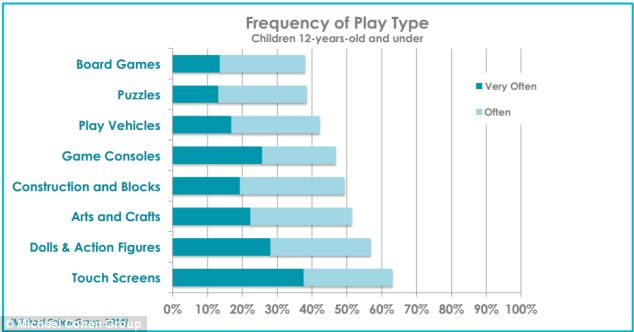
\includegraphics[width=10cm, height=7cm]{immagini/touch.png}
\caption{Time spent by children at playing games}\label{fig:timegames}
\end{figure}
Despite this kind of behaviour is largely criticized and not recommended by doctors and psychologists, the experiment conducted by B. Huber, J. Tarasuik, M.N. Antoniou, C. Garrett, S.J. Bowe and J. Kaufman \cite{Huber} demonstrated that children could learn from touchscreen educational games and apply this knowledge on physical problems. In fact there're a lot of applications thought for this purpose that help children to develop memory, problem-solving and executive functioning skills that could then be applied to real-world problems. The experiment shows substantially that there's no difference in learning for children that use real objects from those who learn only on touchscreen application. In particular, as observed by M.J. Mayo \cite{Mayo}, games could involve children more easily due to the presence of images, animations and sounds. Moreover, they're particularly adept at dosing information delivery. On a touchscreen application it is easy to complicate things and to add visual elements as the difficulty increases, while mantaining the focus on a small area that avoid extraneous distractions, so these educational games seems to be effective in enhancing motivation and increasing children interest in subject matter that leads to more effective learning \cite{Annetta}. 
\section{Google Chromecast}
\section{Projects about food education}
In the specific field of food education, we could find different kinds of game developed for touchscreen devices. In particular one example is the Food pyramid game developed by the Colorado State University \cite{Serrano} as a game to teach children what are the five main food groups and how to apply this knowledge to plan meal and snacks in order to increase their self-efficacy. This game is composed by various challenges regarding the food pyramid, and the researches has concluded that a game composed with a challenge is more effective that one based on a storyline.

